\chapter{システムの線形性とその同定}
対象とするシステムのモデルを作成することで,直接力を測定することなく他のセンサの値から力を推定することが可能である.
前章で導出した物理モデルにおいて未知パラメータを同定すればモデルの構築は可能である.
しかし,バルクや粘性項などのパラメータは温度や圧力などに依存しており,これらのパラメータを正確にしること,そしてすべてのパラメータを同定してモデルを組み上げることは現実的には難しい.

そこで本章ではシステム同定を用いて油圧システムのモデルの構築を行う.
システム同定にあたっては入出力関係を見て同定を行うため,未知パラメータを一つ一つ同定することなくモデルの作成を行うことが可能である.
そこで,バルブへの電圧入力からシリンダ先端の位置及び先端で発生する力までのモデルを,システム同定を用いて導出する.
力の同定ではシリンダ先端を固定した状態で同定をする.
位置の同定にあたっては無負荷状態で行う.
%同定にあたってはシステムの周波数応答を調べて特徴を把握したのちに最小自乗法によるモデルの同定,およびM系列を用いた同定を行いそれぞれを比較する.
\section{実験機とその構成}
本研究で使用する油圧システムの実験装置を\figname\ref{fig:}に示す.
本装置は片ロッドの油圧シリンダ,ギヤポンプ,サーボバルブなどにより構成されており,シリンダにはワイヤー式エンコーダとロードセルが取り付けてある.
また,圧力センサをサーボバルブのAポートおよびBポート,そしてシリンダのヘッド側とロッド側の入り口の計4箇所に取り付けてある.
\begin{figure}[t]
    \centering
        
\includegraphics[keepaspectratio, scale=1.0]{contents/システム同定/figure/3-4ExperimentSystem.png}
        \caption{caption}
        \label{fig:figlabel}
\end{figure}

コントローラ側はPC及びAD/DA変換器やカウンタで構成されており,実験装置に取り付けてあるセンサからの値の取得及びサーボバルブへの入力を行うことができる.
センサ値の処理やサーボバルブへの入力をするための制御アルゴリズムはPC上でMATLAB/Simulinkを用いて組んでいる.
本装置に用いている各部品の諸元をTable~\ref{tab:configuration-parameter}にまとめる.
また,システムの伝達経路の全体像は\figname\ref{fig:}のようになる.
\begin{table}[t]
    \centering
    \begin{tabular}{cccc}
        \hline
        Name & Maker & Model Number & Property\\ \hline \hline
        Servo Valve & nachi & J869-1000A & --- \\
        Hydraulic Cylinder & SMC & CHN-25-250 &     \begin{tabular}{l}internel diameter: \SI{25}{mm} \\ rod diameter: \SI{12}{mm}\end{tabular}\\
        Gear Pump & --- & --- &rated power\SI{7}{Mpa},\SI{2}{l/min} \\\hline
        Load Cell & KYOWA & LUK-A-10kN & ---\\
        Pressure Sensor & KEYENCE & GP-M250? & --- \\
        Encoder & Micro Tech Labolatory & & --- \\ \hline
    PC & mouse computer & --- & \begin{tabular}{l}cpu:i7-7900K \\ gpu:\\OS:windows 10 education\end{tabular} \\
    \begin{tabular}{l}AD/DA Converter \\ Counter\end{tabular}
    & Speedgoat & Speedgoat & --- \\ 
    MATLAB/Simulink & MathWorks & 2018b & --- \\ \hline \hline
    \end{tabular}
    \caption{Experiment System Configuration}
    \label{tab:configuration-parameter}
\end{table}


\section{先端で発生する力までの線形性とモデルの同定}
\label{sec:力までの同定}
バルブへの入力から先端で発生する力までのシステム同定にあたり,\figname\ref{fig:}に示した伝達経路を\figname\ref{fig:system_dentatsu}のように書き直す.
$\mathrm{input}$はコントローラからバルブへの電圧指令,$\fthr$はシリンダの圧力および受圧面積より算出される推力,$f_\mathrm{output}$は実際に先端で発生する力である.
推力$\fthr$は\eqnname\ref{eq:fthr}により算出される.
\begin{align}
    \label{eq:fthr}
    \fthr = \Ah * \phs - \Ar * \prs
\end{align}
ここで$\Ah$はヘッド側の受圧面積,$\Ar$はロッド側の受圧面積,$\phs$はシリンダのヘッド側の圧力,$\prs$はシリンダ側のロッド側の圧力である.
なお,先端で発生する力とはロードセルにより測定された実測値であり,今後これを実測出力と呼ぶ.
\begin{figure}[t]
    \centering
        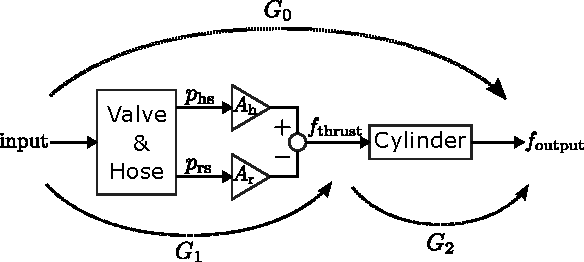
\includegraphics[keepaspectratio, scale=1.0]{contents/システム同定/figure/system_dentatsu.pdf}
        \caption{system}
        \label{fig:system_dentatsu}
\end{figure}

\subsection{線形性調査}
\label{sec:線形性調査(力)}
バルブへの入力に対するシステムの物理量の応答の線形性について調べ,システムの特性の把握を行う.
対象とする物理量は,実測出力$\fmsr$およびシリンダに取り付けてあるヘッド側圧力$\phs$,ロッド側圧力$\prs$である.

バルブへ正弦波入力を与えた際の応答をフーリエ変換し,そのピークが入力した正弦波の角速度と一致し,かつその他の角速度でピークが立たない場合に線形応答とみなすことができる.
実験では,バルブへ入力する角速度として\SI{0.1778}{rad/s}から\SI{100}{rad/s}まで対数上で等間隔に12等分したものを採用した.
サンプリング周期は\SI{0.001}{s}であり,センサから取得される値にはローパスフィルタ(以降LPF)として一次遅れの伝達関数${1}/(0.005s+1)$を通している.
また,直流成分をフーリエ変換を施す前に除去し,フーリエ変換後には角速度のピークに着目するため,最大ピークで除すことで正規化している.

各物理量の応答を\figname\ref{fig:1018FFT_fmeasure}から\figname\ref{fig:1018FFT_prs}に示す.
これより最大ピークの角速度と入力した正弦波の角速度が一致しているため,これらの物理量の応答は線形であるとみなすことができる.
よって対象とする油圧システムは線形なシステムとして扱い,同定することが可能である.
\begin{figure}[t]
    \centering
        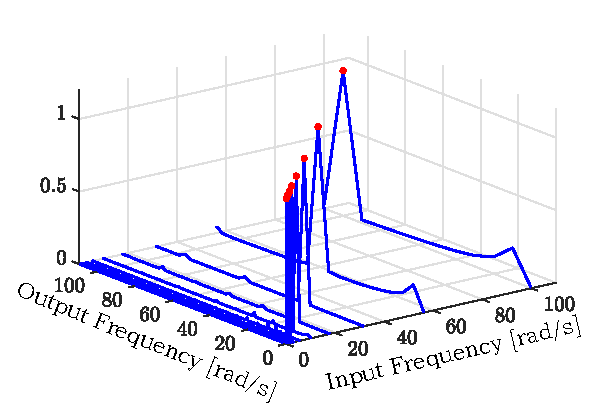
\includegraphics[keepaspectratio, scale=1.0]{contents/システム同定/figure/1018FFT_fmeasure.pdf}
        \caption{FFT of $\fmsr$}
        \label{fig:1018FFT_fmeasure}
\end{figure}
\begin{figure}[t]
    \centering
        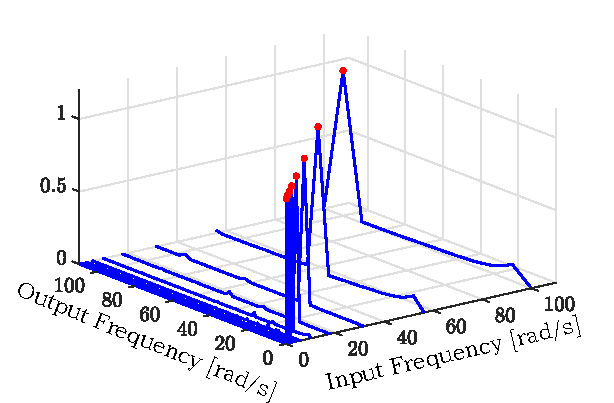
\includegraphics[keepaspectratio, scale=1.0]{contents/システム同定/figure/1018FFT_phs.pdf}
        \caption{FFT of $\phs$}
        \label{fig:1018FFT_phs}
\end{figure}
\begin{figure}[t]
    \centering
        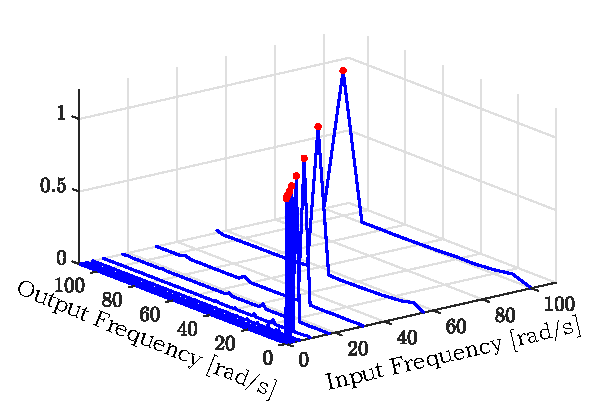
\includegraphics[keepaspectratio, scale=1.0]{contents/システム同定/figure/1018FFT_prs.pdf}
        \caption{FFT of $\prs$}
        \label{fig:1018FFT_prs}
\end{figure}


\subsection{周波数応答と最小自乗法による伝達関数モデルの同定}
入力から実測出力$\fmsr$および推力$\fthr$までのシステムを同定するにあたり,はじめに周波数応答を調べ,システムの特性を把握する.
%入力から実測出力までの周波数応答を調べてシステムの特性を把握し,最小ジオ傑法により伝達関数モデルの同定を行う.
バルブへの入力に\ref{sec:線形性調査(力)}節と同様に正弦波入力を角速度を\SI{0.1778}{rad/s}から\SI{100}{rad/s}まで対数上で等間隔に12等分したものを与え,その際の実測出力$\fmsr$の振幅比と位相遅れをプロットすると\figname\ref{fig:crop-1018_manubode_in2fmea_7MPa}のようになる.
また,バルブへの入力から推力$\fthr$までの周波数応答は\figname\ref{fig:crop-1018_manubode_in2fthr_7MPa}のようになる.
\begin{figure}[t]
    \centering
        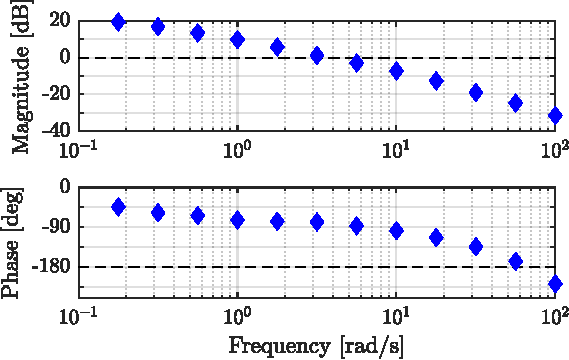
\includegraphics[keepaspectratio, scale=1.0]{contents/システム同定/figure/crop-1018_manubode_in2fmea_7MPa.pdf}
        \caption{Frequency Response from Input to $\fmsr$ (\SI{7}{MPa})}
        \label{fig:crop-1018_manubode_in2fmea_7MPa}
\end{figure}
\begin{figure}[t]
    \centering
        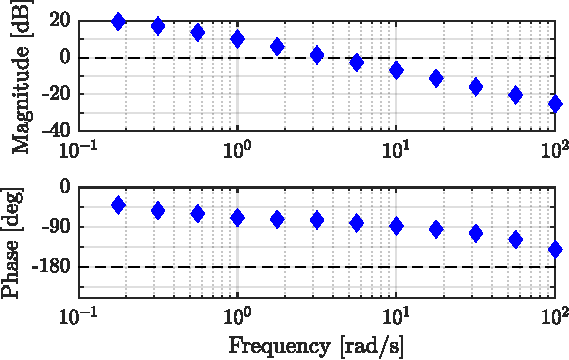
\includegraphics[keepaspectratio, scale=1.0]{contents/システム同定/figure/crop-1018_manubode_in2fthr_7MPa.pdf}
        \caption{Frequency Response from Input to $\fthr$ (\SI{7}{MPa})}
        \label{fig:crop-1018_manubode_in2fthr_7MPa}
\end{figure}

\figname\ref{fig:crop-1018_manubode_in2fmea_7MPa}により,入力から実測出力$\fmsr$までのシステムは\eqnname\ref{eq:tf_est_model}で表されるムダ時間を含む二次遅れ系であると判断した.
\begin{align}
    \label{eq:tf_est_model}
    \GinTofmsr = \frac{a}{(s+b)(s+c)}\mathrm{e}^{-ds}
\end{align}
\eqnname\ref{eq:tf_est_model}の周波数応答が\figname\ref{fig:crop-1018_manubode_in2fmea_7MPa}と一致するように最小自乗法を用いて係数を決定すると,\eqnname\ref{eq:tf_in2fmsr}となる.
\begin{align}
    \label{eq:tf_in2fmsr}
    \GinTofmsr = \frac{41.82}{(s+0.34)(s+130)}\mathrm{e}^{-0.016s}
\end{align}

同様に,入力から推力$\fthr$までの応答はムダ時間を含む一次遅れ系であるとし,その係数を求めると,\eqnname\ref{eq:tf_in2fthr}となる.
\begin{align}
    \label{eq:tf_in2fthr}
    \GinTofthr = \frac{3.4}{s+0.34}\mathrm{e}^{-0.01s}
\end{align}
よって,推力$\fthr$から実測出力$\fmsr$までの伝達関数は\eqnname\ref{eq:tf_in2fmsr}と\eqnname\ref{eq:tf_in2fthr}より\eqnname\ref{eq:tf_fthr2fmsr}となる.
\begin{align}
    \label{eq:tf_fthr2fmsr}
    \GfthrTofmsr = \frac{123}{s+130}\mathrm{e}^{-0.006s}
\end{align}
%\subsection{最小自乗法による伝達関数モデルの同定}
\section{位置までの同定}
\label{sec:位置までの同定}
バルブ入力からシリンダ位置までの応答のモデルの同定を行う.
本節ではシリンダ先端を拘束せず,自由に動く状態で同定を行う.

油圧シリンダにおける入力から位置までの同定は,線形な応答を前提に同定入力として正弦波の足し合わせを入力したもの\cite{ling2012system,zheng2009application}や,M系列による同定を行っているもの\cite{松本貴夢20166,松本貴夢2016},パラメータ同定を行っているもの\cite{前島祐三2011}がある.
本論文でははじめに,対象としている実験機のシリンダの応答の線形性を調べ,前節と同様に最小自乗法による周波数領域での同定,そしてM系列による同定を行う.
\subsection{線形性調査}
バルブに正弦波入力を与え,位置の応答をフーリエ変換してピークを見ることにより線形性を調べる.
入力する正弦波の角速度は\ref{sec:線形性調査(力)}節と同様に\SI{0.1776}{rad/s}から\SI{100}{rad/s}までを対数上で等間隔に12等分したものを与える.

位置までの応答をフーリエ変換した結果を\figname\ref{fig:crop-pos_FFT}に示す.
\figname\ref{fig:crop-pos_FFT}において,入力した正弦波よりも低周波の部分でピークが立っており,応答は厳密には線形応答とは言えない.
本論文においてモデルを得たい領域は比較的低周波の領域であり,正弦波入力の角速度が\SI{50}{rad/s}以下の領域ではピークが大きくなく線形として扱える.
また先行研究において,線形システムとして同定を行った場合でも良い結果が得られていることなどより,本論文においても線形応答の対象としてシステムの同定を試みる.
\begin{figure}[t]
    \centering
        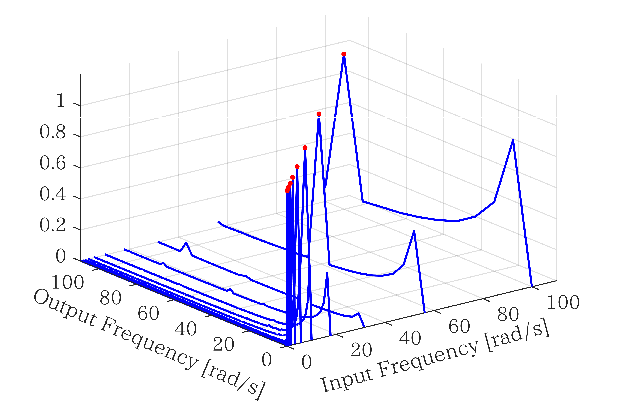
\includegraphics[keepaspectratio, scale=1.0]{contents/システム同定/figure/crop-pos_FFT.pdf}
        \caption{FFT of Input to Position}
        \label{fig:crop-pos_FFT}
\end{figure}

\subsection{周波数応答と最小自乗法によるモデル同定}
位置の応答までの周波数応答を\figname\ref{fig:pos_FR_mea-crop}に示す.
このときのポンプ圧力は\SI{7}{MPa}である.
\figname\ref{fig:pos_FR_mea-crop}より位置までの応答は積分器と一次遅れとムダ時間を含むシステムであると判断でき,最小自乗法により伝達関数モデルを求めると\eqnname\ref{eq:tf_input2pos}となる.
\begin{align}
    \label{eq:tf_input2pos}
    \GinTopos = \frac{330}{s(s+60)}\mathrm{e}^{-0.002s}
\end{align}
\begin{figure}[t]
    \centering
        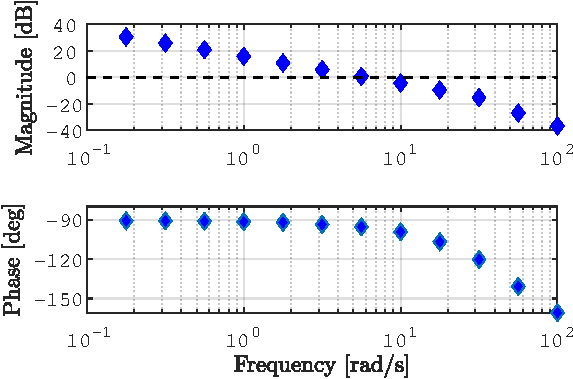
\includegraphics[keepaspectratio, scale=1.0]{contents/システム同定/figure/pos_FR_mea-crop.pdf}
        \caption{Frequency Response from Input to Position}
        \label{fig:pos_FR_mea-crop}
\end{figure}

\clearpage
\begin{figure}[t]
    \centering
        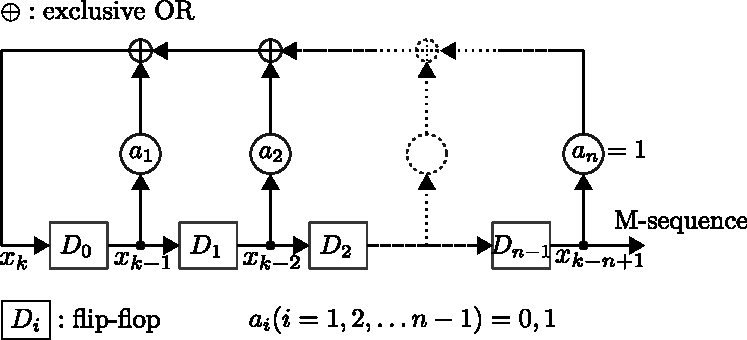
\includegraphics[keepaspectratio, scale=1.0]{contents/システム同定/figure/Mseq.pdf}
        \caption{Generating Circuit of M-sequence}
        \label{fig:Mseq}
\end{figure}

\section{M系列による同定}
\ref{sec:力までの同定}節および\ref{sec:位置までの同定}節では周波数領域で最小自乗法を適用することにより,伝達関数モデルを得た.
本来,対象とするシステムの正確なモデルを得るためには白色雑音を入力として用いることが望ましいが,現実的に白色雑音の適用は不可能であり,代わりとして擬似白色雑音を用いられる.
疑似白色雑音の一つがM系列と呼ばれる信号系列であり,信号の生成が比較的簡単であるためシステム同定の入力としてよく用いられている\cite{足立200909,柏木濶1998m}.
そこで本節では,同定入力にM系列を用いた場合のシステム同定について述べる.
\subsection{M系列の性質}
M系列とは,\figname\ref{fig:Mseq}に示す回路により生成される,0と1から構成される擬似白色雑音である.
\figname\ref{fig:Mseq}は$n$段のシフトレジスタの各段の値に係数$a_i$を掛けてフィードバックし,排他的論理和を適用させる構成になっている.
最初,シフトレジスタの各段には0または1の値が格納されており,全て0でなければその組み合わせは任意である.
これにより発生するM系列は以下の特徴をもつ\cite{吉谷清澄1971pn,近藤勝也2004m,柏木濶1981m}.
\begin{itemize}
    \item 周期系列であり,系列長は$p=2^n-1$である.(周期性)
    \item 1周期内に0は$2^{n-1}-1$個,1は$2^{n-1}$個存在する.(均一性)
    \item 1周期内において連続した$n$個の要素に着目したとき,そのビットパターンは全ての値が0である場合を除く全てのパターンが現れる.
    \item M系列中の1を+1に,0を-1に対応させると,自己相関関数$\phi_j$は\eqnname\ref{eq:mseq-autocorec}のようになる.$j$は元の系列をシフトさせる数である.
    \begin{align}
        \label{eq:mseq-autocorec}
        \phi_j = 
        \begin{cases}
            \displaystyle
            1~&\mathrm{for}~j\equiv0~(\mathrm{mod}~p)\\
            \tfrac{-1}{p}~&\mathrm{for}~j\not\equiv0~(\mathrm{mod}~p)
        \end{cases}
    \end{align}
\end{itemize}
\subsection{システム同定(入力から力)}
バルブへの入力から力までの同定についてM系列を用いての同定を行う.
M系列を用いるさいのサンプリング周波数は,バンド幅の10倍程度に設定するのがよいため\cite{足立200909},\figname\ref{fig:crop-1018_manubode_in2fmea_7MPa}を参考にして,サンプリング時間\SI{0.2}{s}とし,シフトレジスタの個数$n$は8とした.

バルブへの入力と,力の入出力関係を\figname\ref{fig:1018Mseq_inputToFmea}に示す.
\figname\ref{fig:1018Mseq_inputToFmea}のうち,10$\sim$\SI{70}{s}を同定用のデータとして(\figname\ref{fig:1018Mseq_inputToFmea_10-70}),72$\sim$\SI{100}{s}を検証用データとして(\figname\ref{fig:1018Mseq_inputToFmea_72-100})用いる.

同定した伝達関数$\GinTofmsr$は,\eqnname\ref{eq:tf_mseq_force}であり,分子第2項および分母第3項を微小として無視し整理すると,\eqnname\ref{eq:tf_mseq_force_hosei}となる.
\begin{align}
    \label{eq:tf_mseq_force}
    \GinTofmsr&=\frac{4.193s+0.02265}{s^2 + 1.118s + 7.614\times 10^{-11}}\mathrm{e}^{-0.02s}\\
    \label{eq:tf_mseq_force_hosei} 
    \GinTofmsr&= \frac{4.19}{s+1.12}\mathrm{e}^{-0.02s}
\end{align}
\eqnname\ref{eq:tf_mseq_force}および\eqnname\ref{eq:tf_mseq_force_hosei}の応答と,\figname\ref{fig:1018Mseq_inputToFmea_72-100}の結果を比較すると,\figname\ref{fig:1018Mseq_compare}のようになる.
tf(w/o shaping)が\eqnname\ref{eq:tf_mseq_force}の応答,tf(with shaping)が\eqnname\ref{eq:tf_mseq_force_hosei}の応答である.
それぞれの横に書いてある数字はFit率であり,\eqnname\ref{eq:fit}で算出される適合率の値である.
\begin{align}
    \label{eq:fit}
    \mathrm{Fit} =  \left( 1- \frac{\sqrt{\sum_{k=1}^N |\hat{y}(k)-y(k)|^2 }}{\sqrt{\sum_{k=1}^N |{y}(k)-\bar{y}|^2 }}\right) \times 100
\end{align}
ここで,$y(k)$は実際の出力,$\hat{y}(k)$はモデルの出力,$\bar{y}$は実際の出力の平均値である.
\figname\ref{fig:1018Mseq_compare}より,微小項を無視してもFit率がほぼ下がっていないので\eqnname\ref{eq:tf_mseq_force_hosei}を同定結果として用いても問題ない.
よって\eqnname\ref{eq:tf_mseq_force_hosei}をmodel TD:$\GTD$として扱う.
\begin{align}
    \label{eq:tf_GTD}
    \GTD = \frac{4.19}{s+1.12}\mathrm{e}^{-0.02s}
\end{align}
\begin{figure}[t]
    \centering
        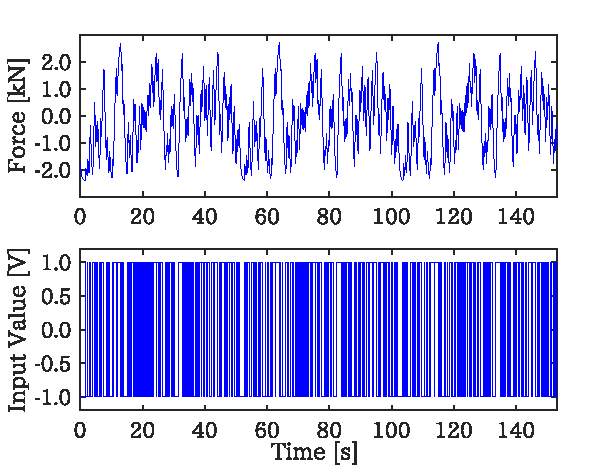
\includegraphics[keepaspectratio, scale=1.0]{contents/システム同定/figure/1018Mseq_inputToFmea.pdf}
        \caption{Input and Output Data}
        \label{fig:1018Mseq_inputToFmea}
\end{figure}
\begin{figure}[t]
    \centering
        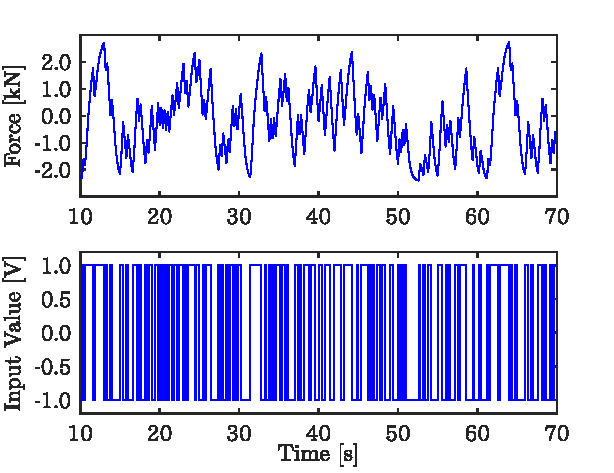
\includegraphics[keepaspectratio, scale=1.0]{contents/システム同定/figure/1018Mseq_inputToFmea_10-70.pdf}
        \caption{Input and Ooutput Data for System Identification}
        \label{fig:1018Mseq_inputToFmea_10-70}
\end{figure}
\begin{figure}[t]
    \centering
        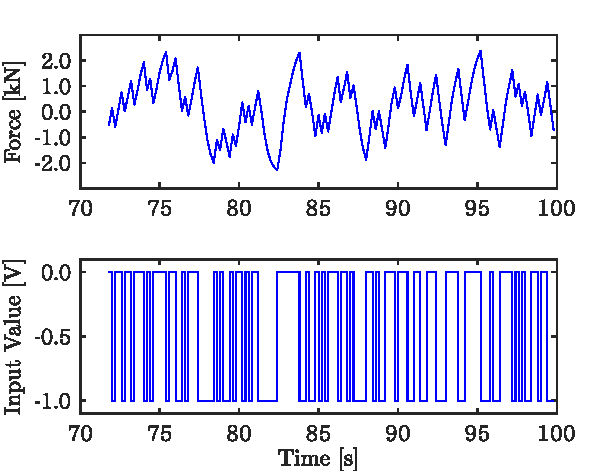
\includegraphics[keepaspectratio, scale=1.0]{contents/システム同定/figure/1018Mseq_inputToFmea_72-100.pdf}
        \caption{Input and Ooutput Data for System Identification}
        \label{fig:1018Mseq_inputToFmea_72-100}
\end{figure}
\begin{figure}[t]
    \centering
        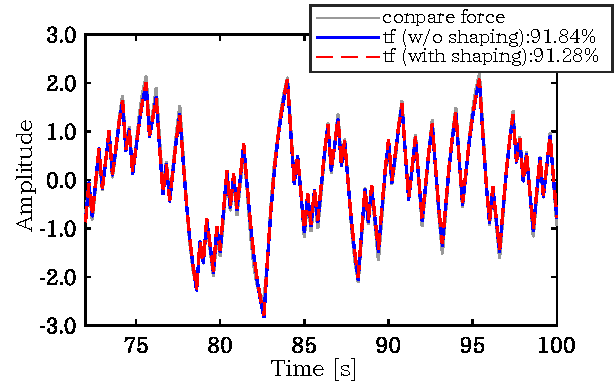
\includegraphics[keepaspectratio, scale=1.0]{contents/システム同定/figure/1018Mseq_compare.pdf}
        \caption{Compare data}
        \label{fig:1018Mseq_compare}
\end{figure}

\subsection{システム同定(入力から位置)}


















